\chapter{ローカルデータベースに実装した読み出し試験結果検索機能の詳細と処理時間測定}

生産時には、読み出し試験の結果は一つの機関で大量に生じるものである。
4章で述べたように、任意のタイミングで必要な結果を取得できる検索機能を実装した。詳細について以下に示す。


\section{実装方法}
今回の実装では、一般的にウェブで用いられているフリーワードの検索エンジンのような機能を実装しようと考えた。
ユーザの操作を最小限にし、柔軟な検索ができるようにするためである。

読み出し試験において、対象とする検索キーワードを以下の項目に絞った。
システムにおいて、アップロードされた試験結果に関わるデータベース内の情報は固定されていて、試験結果情報の変更はしないことを前提としている。
そのため、ユーザが対象としたい検索キーワードは以下の項目に限られ、検索キーワードとして以下の項目をサポートすれば十分であると考えた。

\begin{itemize}
  \item モジュール及びFEチップのID
  \item 読み出し試験項目(例:std$\_$digitalscan)
  \item 読み出し試験者
  \item 読み出し試験場所
  \item 試験日時(将来的に範囲指定を用いた検索機能を検討)
  \item タグ機能を用いてつけられたタグ
\end{itemize}

そこで実装方法として、以下の2つを考えた。

\begin{enumerate}
  \item 各試験に関する情報をPythonリスト集め、検索キーワードが含まれるかを確認する方法
  \item 各試験に関する情報を持つドキュメント、コレクションを予め作成、それを参照し検索を行う方法
\end{enumerate}

これらについて以下で詳細を説明する。

\subsection{方法1: Pythonリストを用いた一致確認}
Pythonリストを使う実装の場合、以下のような流れで検索処理を行う。
\begin{enumerate}
  \item ユーザが検索ワードを入力し、処理を実行
  \item 読み出し試験に関する情報を全て取得
  \item Pythonリストに保持、検索ワード一致を確認、試験を選別
  \item ブラウザーに送信
\end{enumerate}

アルゴリズムのイメージを図\ref{search_python_list}に示す。
この方法では、データベース内の試験結果とアプリケーションの関数内だけで全ての処理を行うことが可能なため、シンプルな実装方法である。

\begin{figure}[bpt]
  \begin{center}
    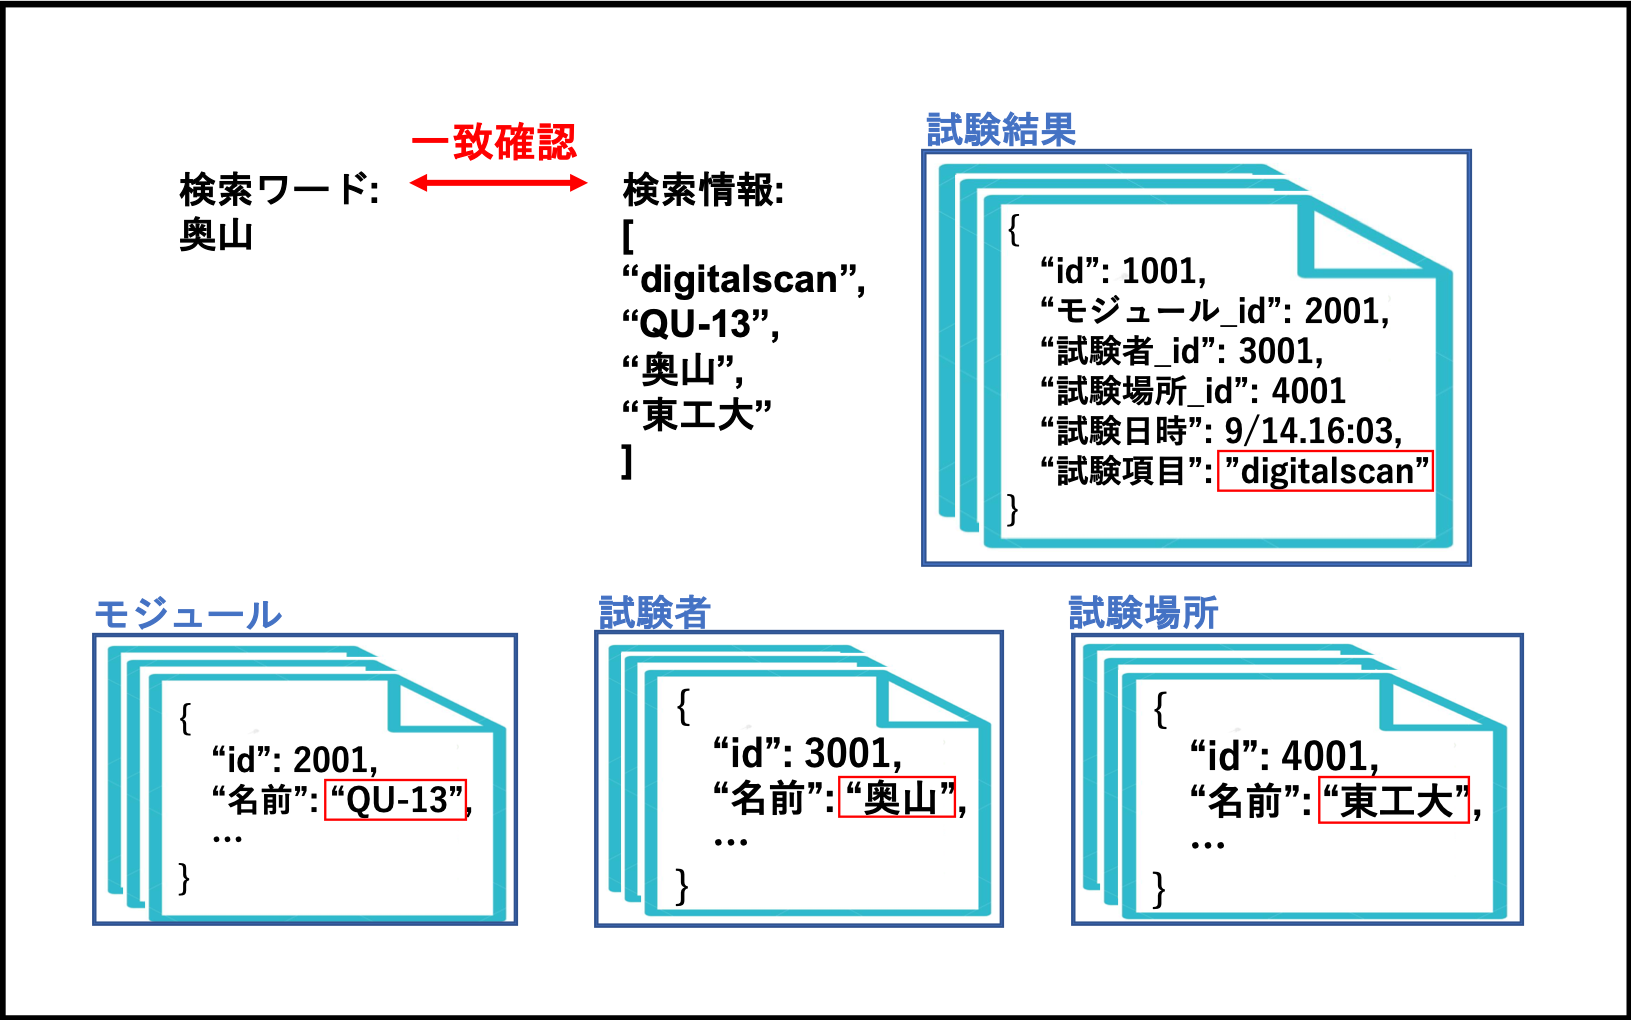
\includegraphics[width=16cm]{search_python_list}
    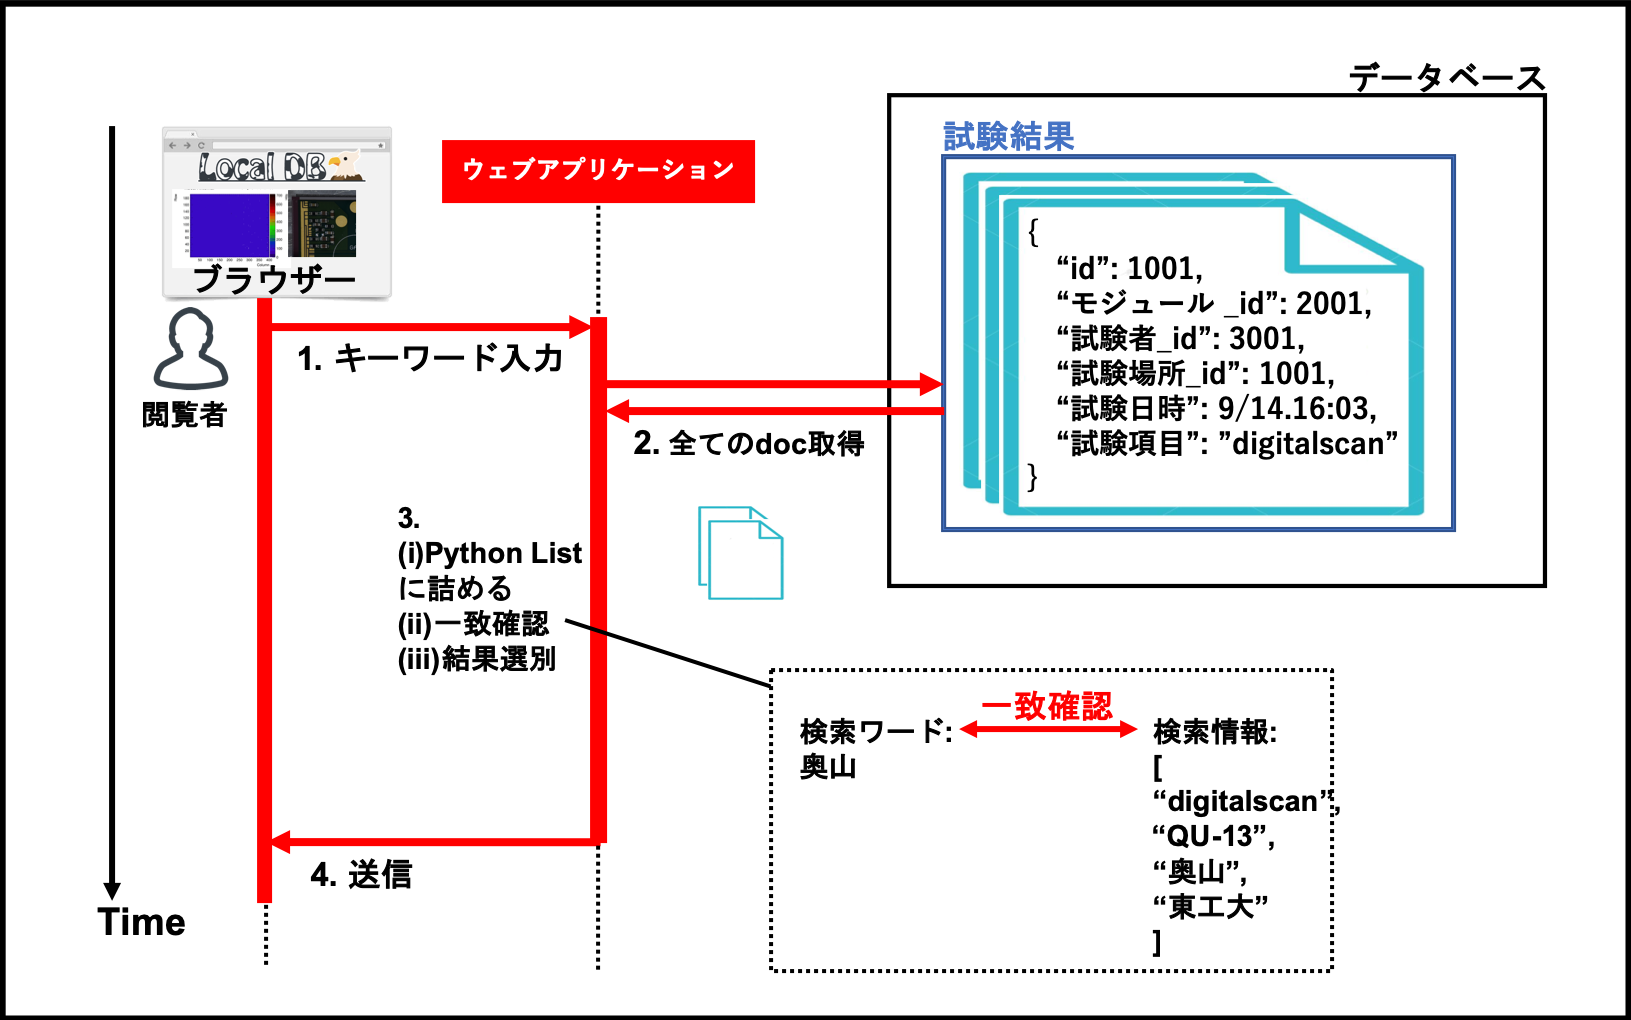
\includegraphics[width=16cm]{search_python_list_flow}
  \caption[検索機能実装方法1:Pythonリストを用いた場合]{検索機能実装方法1:Pythonリストを用いた場合}
  \label{search_python_list}
  \end{center}
\end{figure}

ユーザが処理を実行した際にデータベース内で情報を取得し、Pythonリストにつめる処理を行う。
\\

しかしこの方法を試験実装したところ、データベース内の構造は複雑であり複数のコレクションを跨いで情報を保持しているため、試験結果全てに対してリアルタイムでこの処理を行うと、時間を大きく要してしまう問題が発生した。
イメージを図\ref{search_python_list_problem}に示す。

このシステムにおいては試験結果数を$n$とすると、試験結果情報を保存しているtestRun、componentとtestRunの関係を保存するcomponentTestRunがぞれぞれ$O(n)$のドキュメント数を持つことになる。
各componentの情報を取得し、一致確認を行うと$O(n^2)$の時間がかかる。イメージを図\ref{search_python_testRun}に示す。


\begin{figure}[bpt]
  \begin{center}
    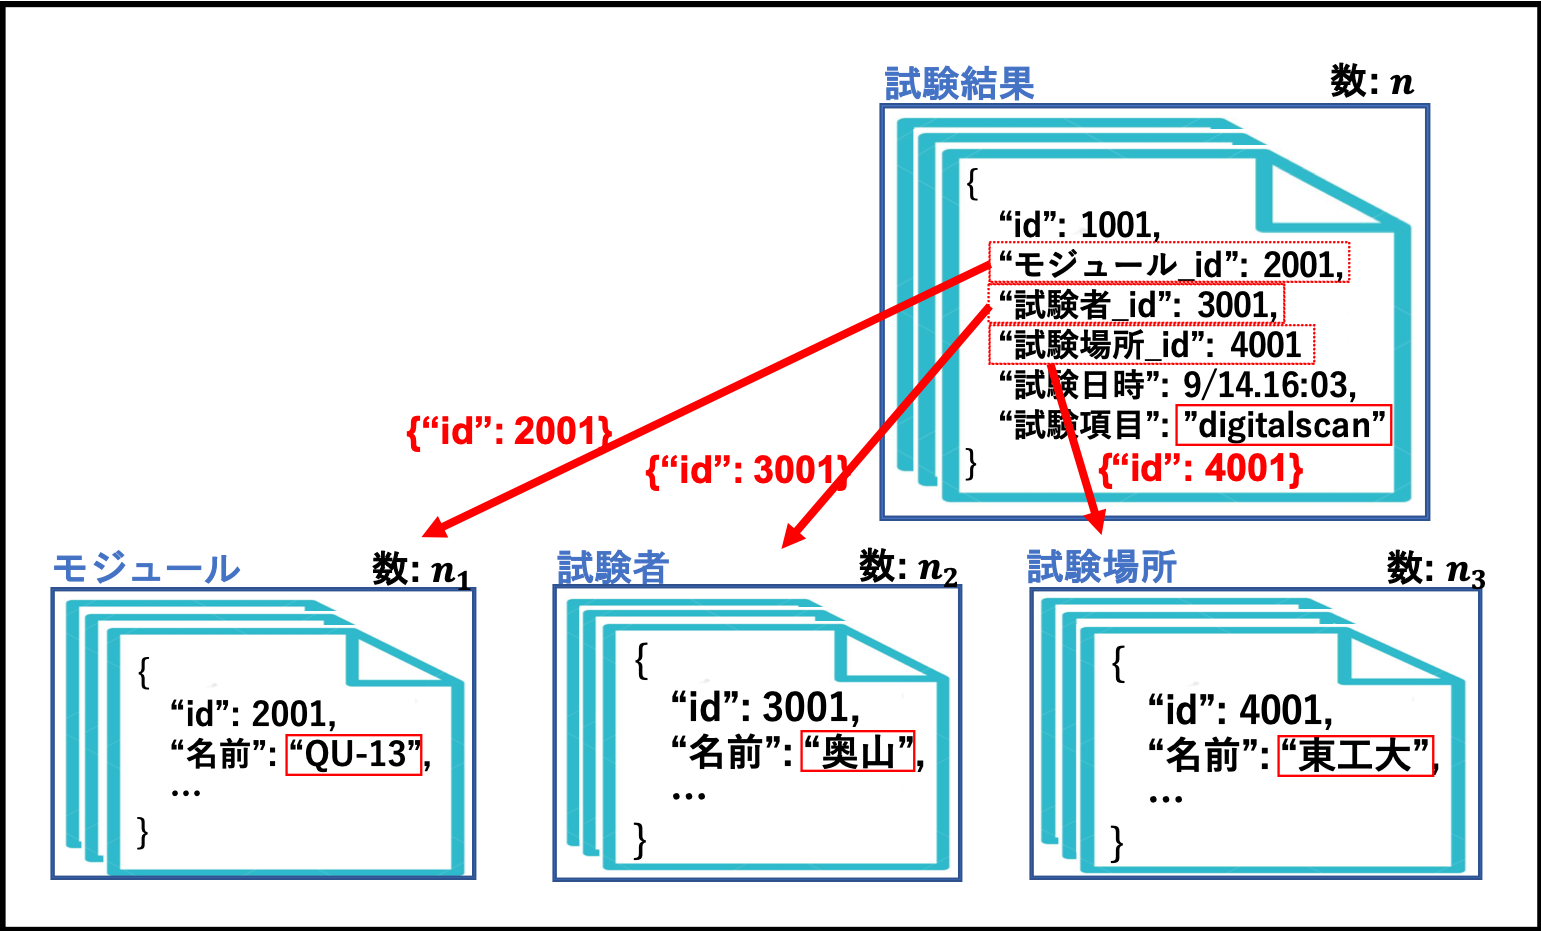
\includegraphics[width=16cm]{search_python_list_problem}
  \caption[検索機能実装方法1の問題点]{検索機能実装方法1の問題点}
  \label{search_python_list_problem}
  \end{center}
\end{figure}

\begin{figure}[bpt]
  \begin{center}
    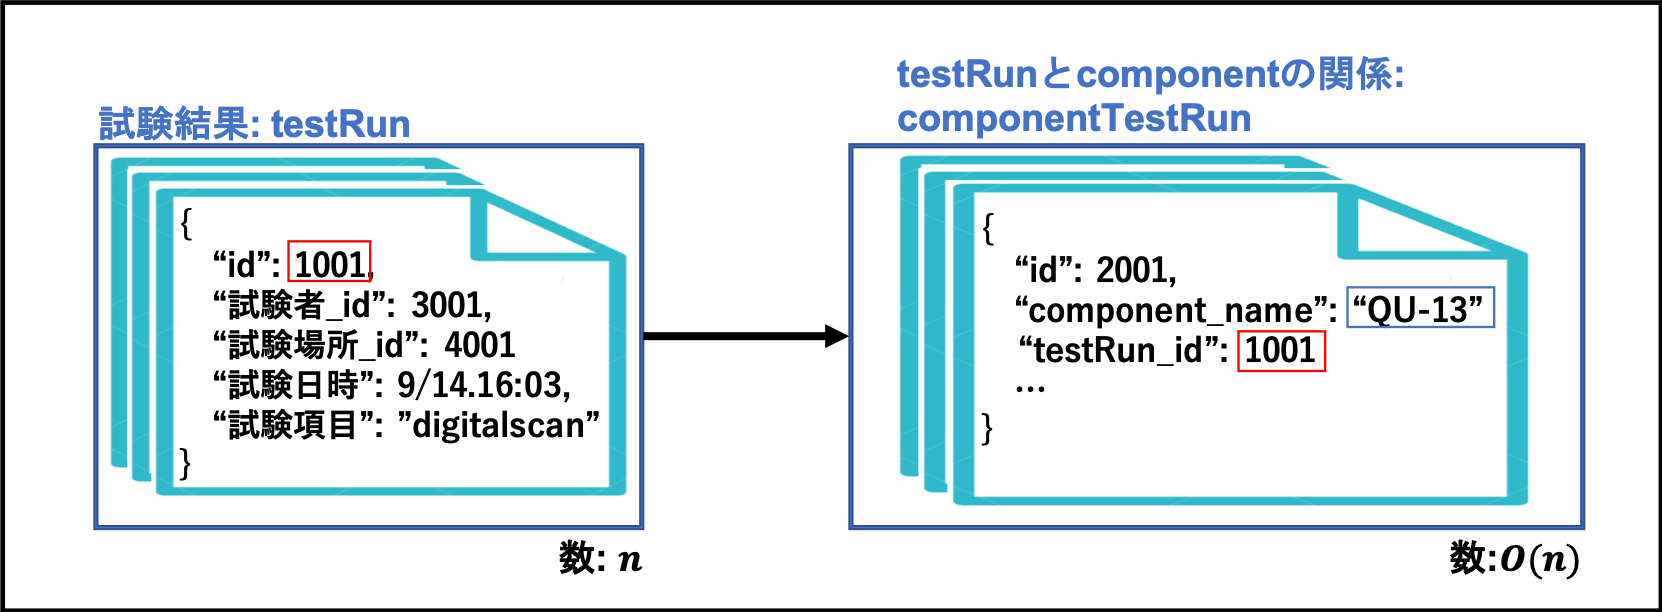
\includegraphics[width=16cm]{search_python_testRun}
  \caption[検索機能実装方法1の問題点詳細]{検索機能実装方法1の問題点詳細}
  \label{search_python_testRun}
  \end{center}
\end{figure}

\subsection{方法2: 検索情報を持つドキュメントを作成、使用}
検索機能を改善するため方法2を考案し、実装を行った。アルゴリズムのイメージを図\ref{search_mongo_collection}に示す。
検索キーワードを別のドキュメントに予め保持しておき、処理実行時にはそれを参照することで検索を行う。
検索情報コレクションに入るドキュメント数は、試験結果数と同じであるため$O(n)$であり、検索コストを削減できると考えた。

\begin{figure}[bpt]
  \begin{center}
    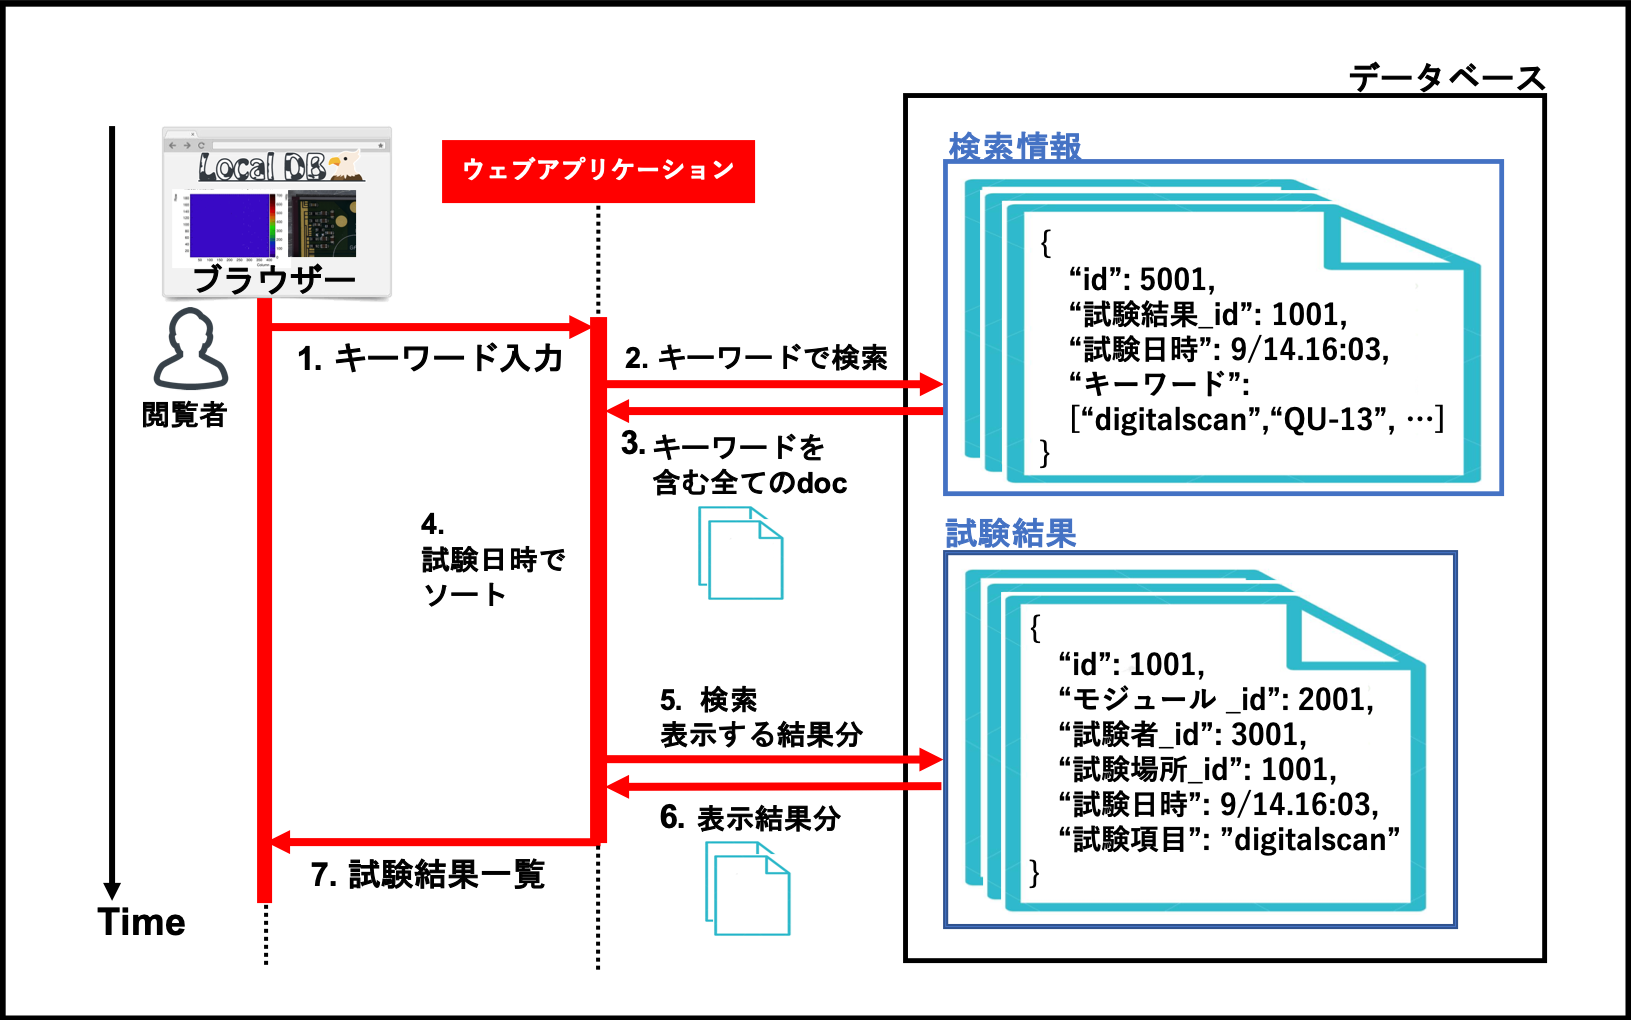
\includegraphics[width=16cm]{search_mongo_collection}
    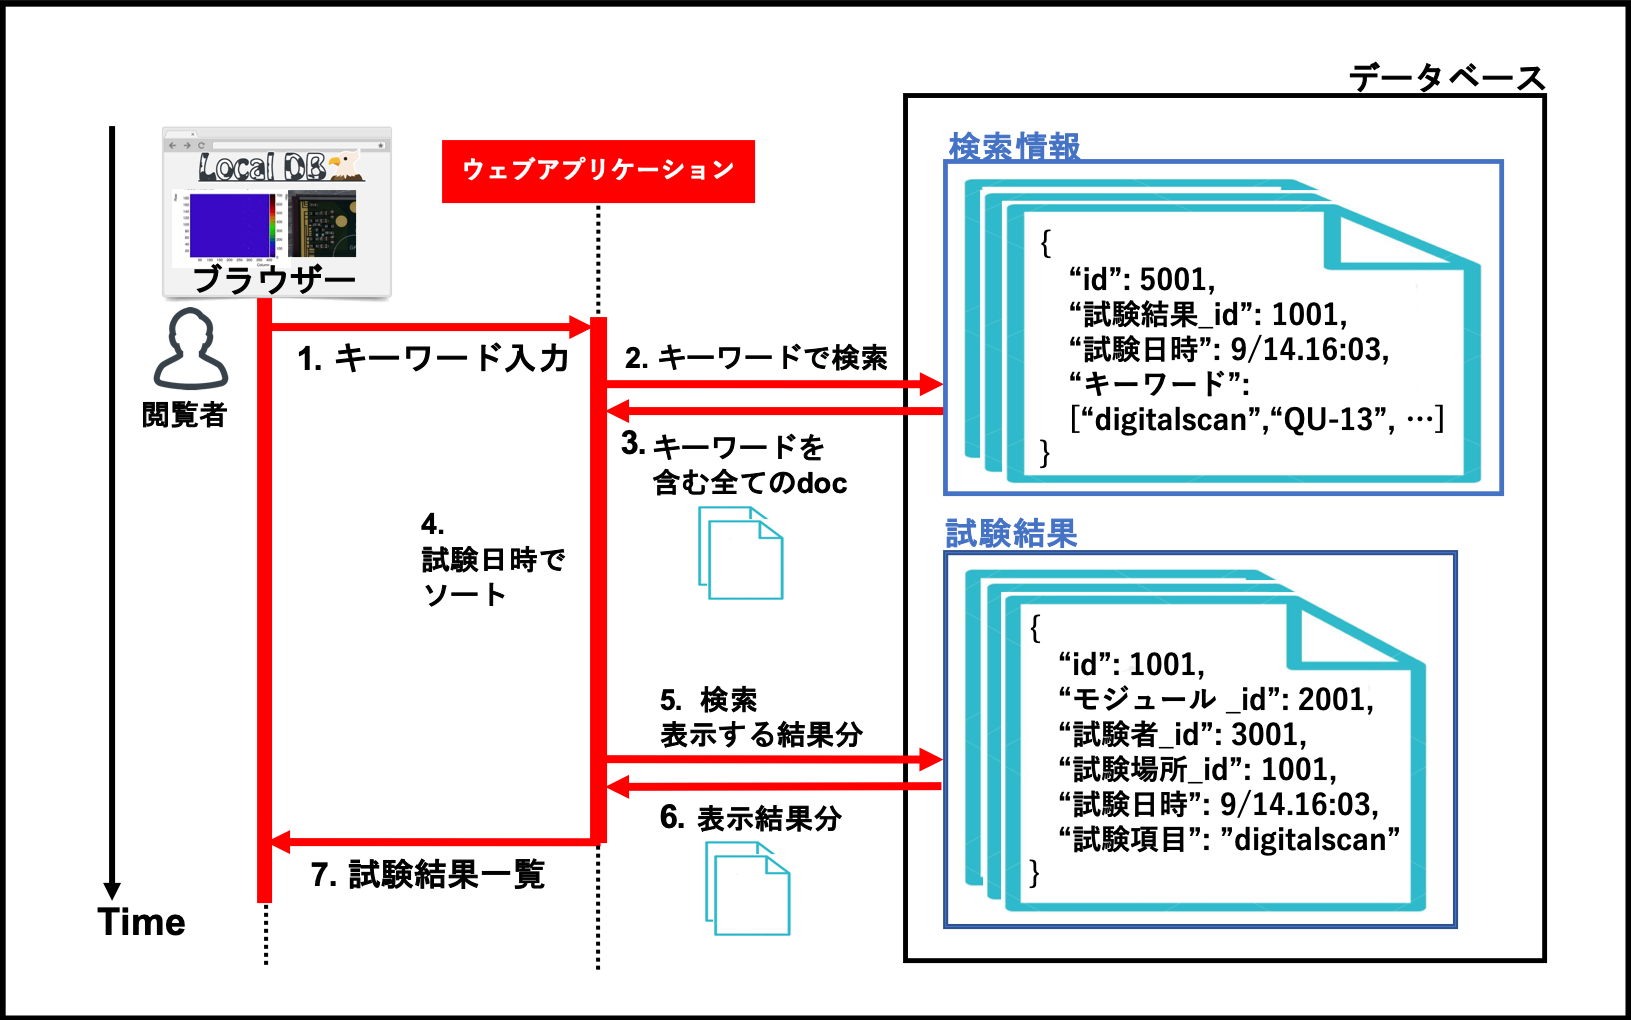
\includegraphics[width=16cm]{search_mongo_collection_flow}
  \caption[検索機能実装方法2:検索キーワード専用コレクションを用いた場合]{検索機能実装方法2:検索キーワード専用コレクションを用いた場合}
  \label{search_mongo_collection}
  \end{center}
\end{figure}

\section{処理時間測定}
先述した方法1と2において、検索処理時間の測定を行った。詳細を以下に示す。


\subsubsection{使用したデバイス}

測定には個人のlaptopPCを用いた。specを表\ref{laptop_spec}に示す。

\begin{table}[tbp]
\caption[laptopの性能]{laptopの性能}
\label{laptop_spec}
\scalebox{0.9}{
  \begin{tabular}{|l|llll|l|l|} \hline
    設置機関 & CPU & & & & Memory & Disk \\
     & Type & Core & Thread & Clock speed[GHz]& [kB] & [GB] \\ \hline 
    CERN & Intel Core Processor (Broadwell, IBRS) & 1 & 10 & 2.2 & 29,978,888 & 80\\ \hline
  \end{tabular}
}
\end{table}


\subsubsection{測定内容}

コマンドプロンプトから以下を使用し、リクエストに対するアプリケーションのレスポンス時間を測定した。
実際にアプリケーションを使用する際には、ブラウザーに一覧表示をする時間が今回の測定時間に加算されることになる。

\begin{lstlisting}
curl "http://127.0.0.1:5000/localdb/scan?keywords=okuyama&match=partial" 
-o /dev/null -w "$\%${time$\_$total}\n" 2> /dev/null -s
\end{lstlisting}

上記のコマンドを用いて、試験結果数に対するレスポンス時間の測定を行った。
測定に関する詳細を表\ref{searching_measurement_details}に示す。

\begin{table}[tbp]
\begin{center}
\caption[検索機能処理時間測定の詳細]{検索機能処理時間測定の詳細}
\label{searching_measurement_details}
\scalebox{0.9}{
  \begin{tabular}{|l|l|} \hline
    試験結果数 & 1, 5000, 10000, 15000, 20000\\
    測定回数 & 各測定点に対して20回\\
    検索キーワード & okuyama\\
    検索モード & 部分一致\\
    各試験結果が持つ検索情報 & 全試験結果に対して同じ、以下に詳細\\\hline
    検索情報一覧             & モジュール名: 20UPGR10000005\\
		                         & FEチップ名:   20UPGTU9000000\\
		                         & 試験項目:     std$\_$digitalscan\\
		                         & 試験者:       okuyama\\
		                         & 試験場所:     default$\_$host\\
		                         & 試験日時:     2020/12/06\\\hline
  \end{tabular}
}
\end{center}
\end{table}


各測定点に対して平均値、標準偏差を算出し、フィッティングを行った。


\subsubsection{測定結果}

結果を図\ref{searching_time}に示す。
方法1に対して、方法2の処理時間は改善されていることが分かる。
現在は方法2で検索機能を実装し、サービスの1つとして提供している。

\begin{figure}[bpt]
  \begin{center}
    
\includegraphics[width=16cm]{figure}
  \caption[検索処理速度測定]{検索処理速度測定}
  \label{searching_time}
  \end{center}
\end{figure}

各方法について、生産時における処理時間の見積もりを行う。簡単のため生産時に使うサーバーのspecとの性能差は考慮に入れない。
hogehogehoge
 
\section{いくつかの改善点と比較}
\subsection{ボトルネックとなっている処理}
mongo findが問題点になっているよ。

\subsection{改善点}
上記の問題点を踏まえ、以下の2つの方法を新しく考え処理時間測定を行った。

\begin{enumerate}
  \setcounter{enumi}{2}
  \item 検索情報のコレクションに一覧表示に必要な情報を保持、参照 
  \item 方法3に付け加えて、検索情報のドキュメントを複数コレクションに分散、マルチスレッド
\end{enumerate}

方法3、4について、アルゴリズムのイメージをそれぞれ図\ref{search_summary_hash}、\ref{search_multi_thread}に示す。

\begin{figure}[bpt]
  \begin{center}
    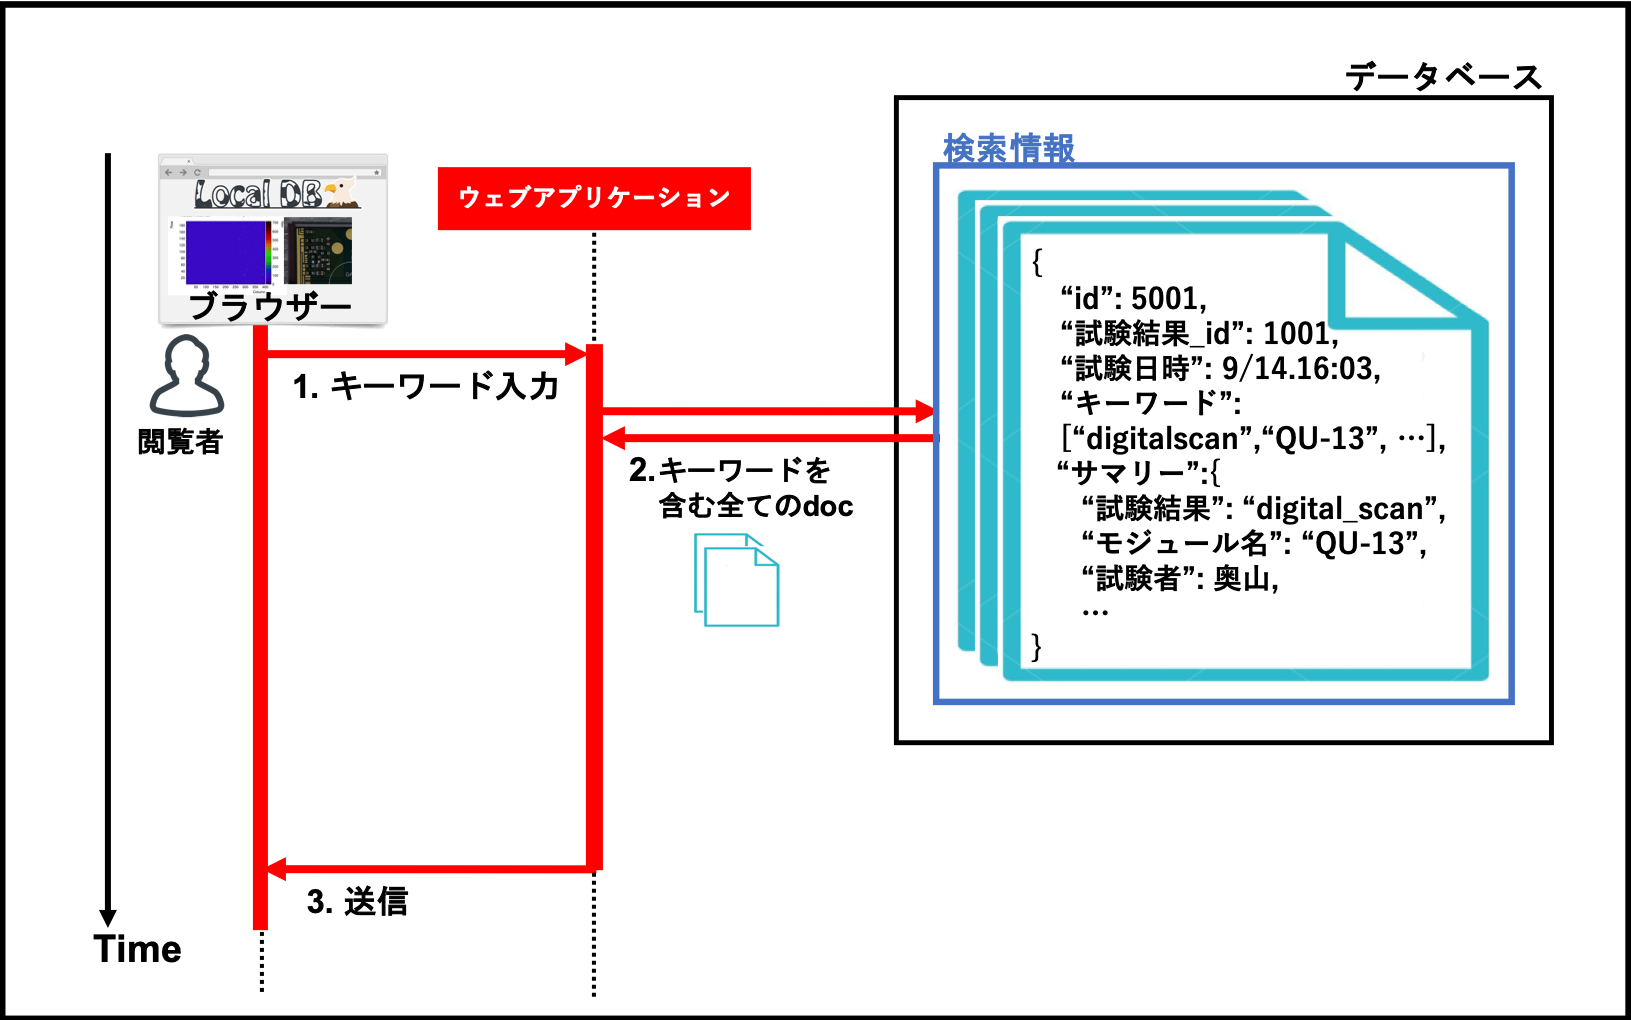
\includegraphics[width=16cm]{search_summary_hash}
  \caption[検索機能実装方法3:検索情報と共に一覧表示に必要な情報を保持]{検索機能実装方法3:検索情報と共に一覧表示に必要な情報を保持}
  \label{search_summary_hash}
  \end{center}
\end{figure}

\begin{figure}[bpt]
  \begin{center}
    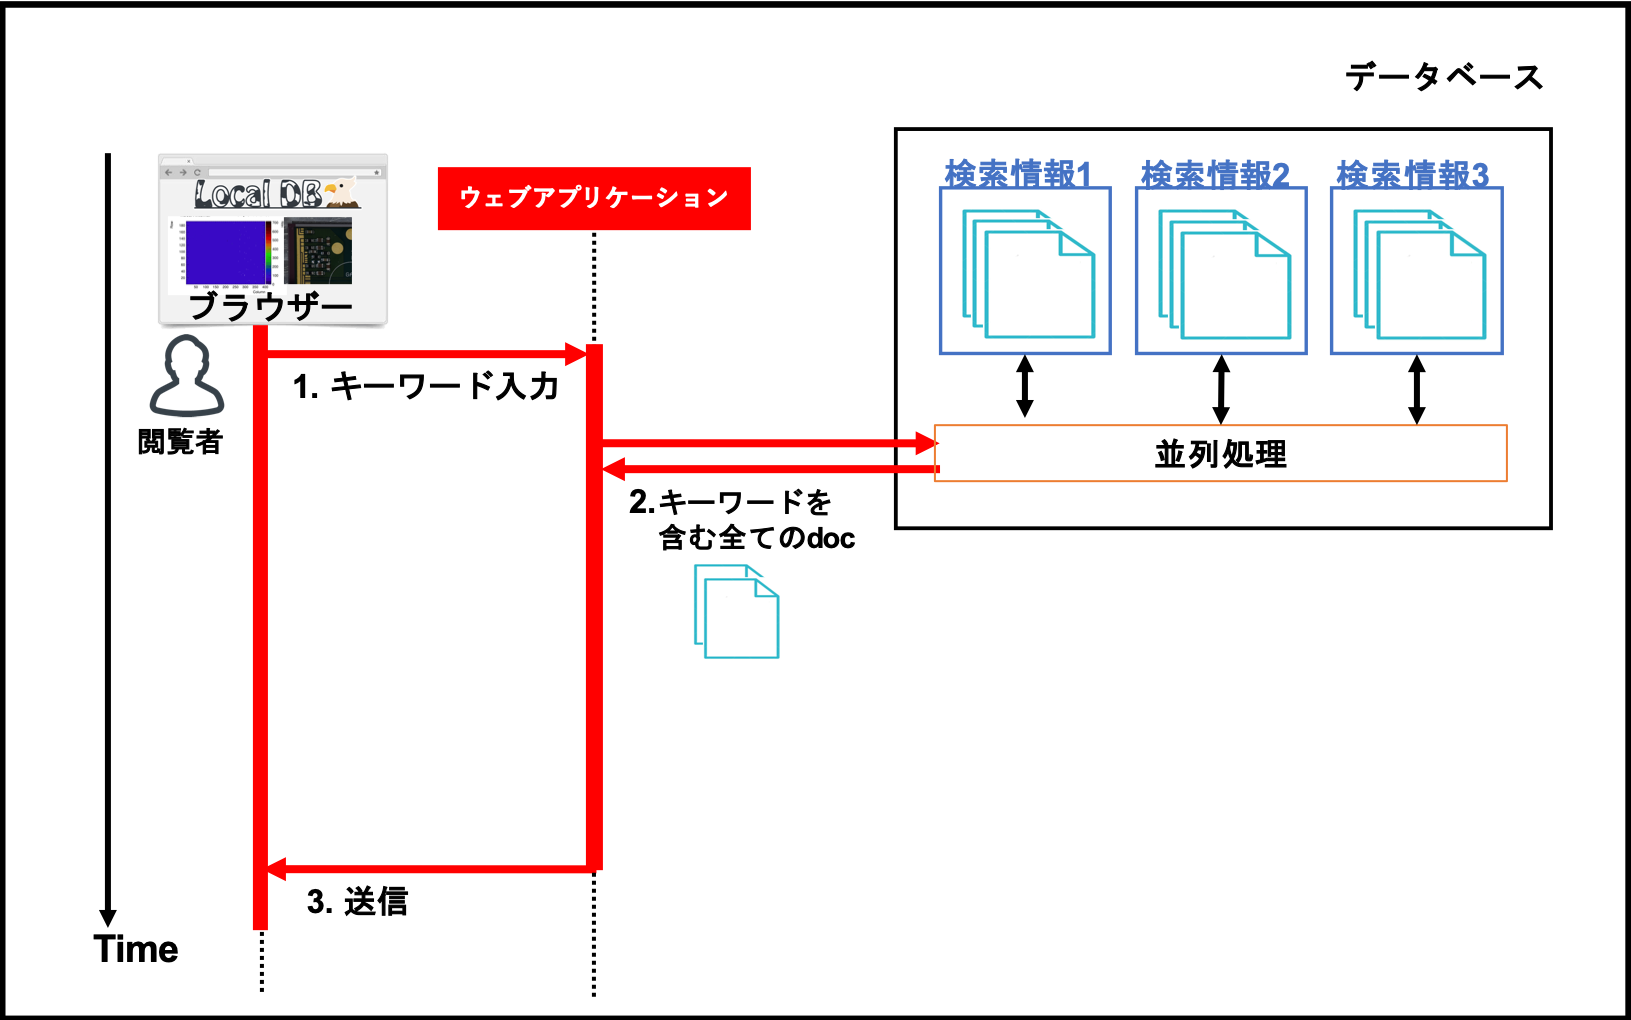
\includegraphics[width=16cm]{search_multi_thread}
  \caption[検索機能実装方法4:検索情報コレクションを分散、マルチスレッドを用いる]{検索機能実装方法4:検索情報コレクションを分散、マルチスレッドを用いる}
  \label{search_multi_thread}
  \end{center}
\end{figure}

